\renewcommand{\theequation}{\theenumi}
\begin{enumerate}[label=\arabic*.,ref=\thesubsection.\theenumi]
\numberwithin{equation}{enumi}
\item  given that $\to$
\begin{align}
Z &= x + 2y
\\
\text{subjected to}
\\
2x + y &\geq 3
\\
x + 2y &\geq 6
\\
x  &\geq 0
\\
y &\geq 0
\end{align}
Comparing above equation to the gernelised form$\to$ 
\begin{align}
miniZ &= c^t \vec{x}
\\
\text{subjected to}
\\
A\vec{x} &\preceq b
\\ 
\text{we can find $\to$ }
\\
c &= \myvec{1\\ 2}
\\
A &= \myvec{2 & 1 \\ 1 & 2}
\\
b &= \myvec{3\\6}
\end{align}\\
Solution for the above equations can be find from the python code of Lenear programing.\\
	\begin{lstlisting}
./optimization/codes/lp8.eps
\end{lstlisting}

From the codes we get that the miniimum value of the equation will be 6 but from the line  eqaution 2 we can see that  it gives 6 on each point thus for minimum  value of 6 there are more than 2 points .

\begin{figure}[!ht]
	\centering
	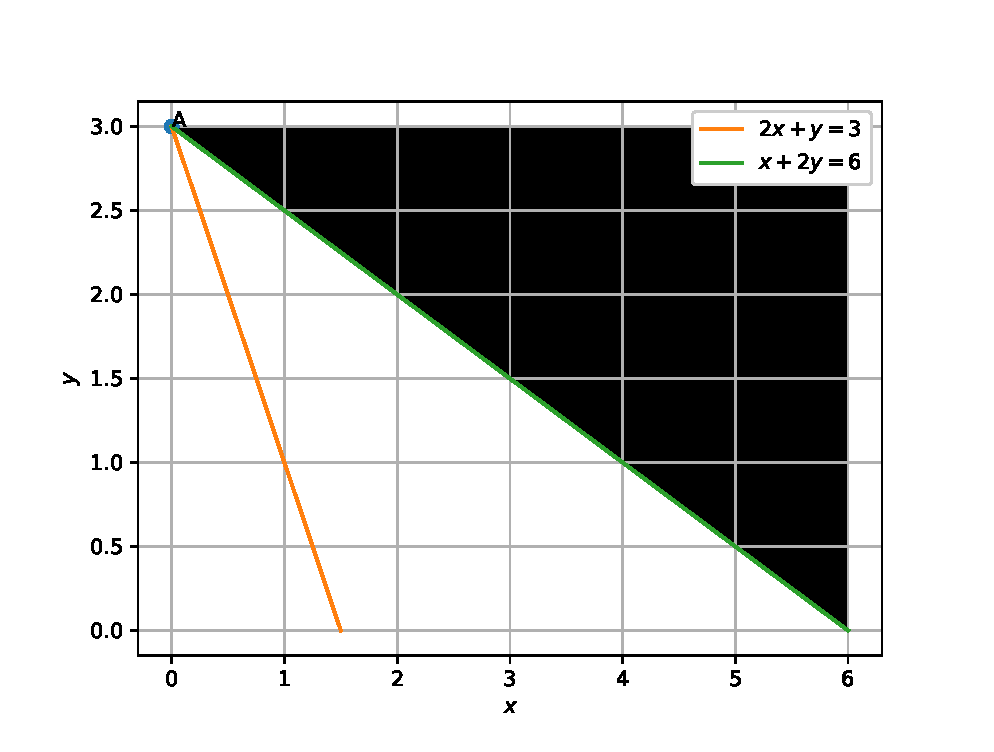
\includegraphics[width=\columnwidth]{./figures/lp8.eps}
	\caption{ lp8}
	\label{fig:lp8}
	Pythone codes for the above figure can be get from
	\begin{lstlisting}
	./optimization/figures/lp8.eps
	\end{lstlisting}	
\end{figure}
\end{enumerate}